	Este capítulo aborda as características de um sistema de arquivos distribuído. 
	%Primeiramente é explanado o que é um sistema  de arquivos, e então, o texto avança apresentando as consequências de tais características no sistema de arquivos de um sistema distribuído.
	

	\section{Sistema de arquivos}
	
	
	O sistema de arquivos é um sistema fundamental que possui papel de gerenciar todos os dados armazenados em um computador.
	Em geral está incluso no sistema operacional, como ocorre nos casos de FAT32 e NTFS para sistema de \textit{Windows} ou EXT4 para sistema de \textit{Linux}.
	%\section{Sistema distribuído}
	%Hoje em dia, podem ser encontradas diversas tarefas computacionais que são impossíveis de ser processadas por um computador comum, devido a simples limitação da capacidade de processamento que uma máquina pode atingir. A solução tipicamente tomada por muitas organizações é o uso de sistemas distribuído, o qual possui algumas vantagens comparado a um sistema centralizado, como pode ser visto a seguir.
	
	%\begin{itemize}
	%	\item Melhor relação custo-benefício;
	%	\item Capacidade de processamento além dos limites práticos de sistema centralizado;
	%	\item Alta confiabilidade e disponibilidade;
	%	\item Relação linear entre crescimento de custo e desempenho.
	%\end{itemize}
	%Os sistemas de computação distribuída são caracterizados pela sua estrutura, que consiste em interação entre um grande número de dispositivos que executam seus próprios programas, mas que são afetados recebendo as mensagens ou observando a memória compartilhada de outros dispositivos.
	%\\
	
	%, os eventos imprevisíveis, como atrasos nas chegadas de mensagem, súbito falhas de componentes, ou em caso extremo, as ações nefastas de defeitos ou máquinas maliciosos que agem opostamente para os objetivos do sistema como um todo.
	
	\subsection{Metadado} 
	
	Os sistemas de arquivos, como ambientes propícios para a recuperação de informações, têm na utilização de metadados a padronização das formas de representação e a possibilidade de garantia de interoperabilidade entre sistemas, favorecendo a integridade e a acessibilidade dos recursos informacionais de forma eficiente pelo usuário final. Os metadados são "dados de dados", ou seja, as informações essenciais sobre os arquivos armazenados, indispensáveis para fazer o gerenciamento de arquivos, indicando as características inerentes deles. A Tabela~\ref{tab:metadado} mostra os atributos tipicamente encontrados em um metadado.
	
	\capstartfalse
	\begin{table} [htb]
		\caption{Elementos de metadados}
		\centering
		\begin{tabular}{|l|l|} \hline
			\textbf{Informação} & \textbf{Descrição} \\ \hline
			
			Nome do arquivo		& O nome do arquivo, incluindo o caminho do diretório.\\ \hline
			Proprietário		& O identificador de usuário que é o dono do arquivo.\\ \hline
			Data de criação     & Data que o arquivo foi criado.\\ \hline
			Data de acesso		& Data de último acesso do arquivo. \\ \hline
			Data de atualização	& Data de última atualização feito sobre o arquivo. \\ \hline
			Tamanho				& Espaço ocupado pelo arquivo ao longo do disco. \\ \hline
			Tipo de arquivo		& indica se ele é uma pasta ou um arquivo normal.  \\ \hline
			Modo de acesso		& indica a permissão para acessar o arquivo. \\ \hline
			Bloqueio			& indica se o arquivo está bloqueado para acesso. \\ \hline
			%Lista de servidores	& lista de todos os servidores que armazena partes do arquivo. \\ \hline
			
		\end{tabular}
		\label{tab:metadado}
	\end{table}
	\capstarttrue
	
	%\subsection{Sistema distribuído}
	
	%Existem várias definições e pontos de vista sobre o que são sistemas distribuídos. Coulouris~\cite{coulouris06} define um sistema distribuído como "um sistema no qual os componentes de \textit{hardware} e \textit{software} localizadas nos computadores conectados por rede comunicam e coordenam suas ações somente por passagem de mensagens", e Tanenbaum~\cite{tanenbaum07} define como "uma coleção de computadores independentes que aparenta ao usuário ser um computador único". Leslie Lamport, um pesquisador sobre sistema distribuído, disse uma vez que "um sistema distribuído é aquele em que é impedido de prosseguir com seu trabalho devido a uma falha de algum computador que nunca ouviu falar" ~refletindo o grande número de desafios enfrentados pelos projetistas de sistemas distribuídos.
	%\\	
	
	%Assim, quando um sistema distribuído aumenta a sua escala, torna-se cada vez mais difícil de prever ou mesmo entender o seu comportamento. 
	%Uma parte da razão para isso é simples falta de ferramentas que gerenciam a complexidade e outra parte é que um sistema distribuído de grande porte traz consigo a quantidade enorme de não-determinismo inerente.
	
	\section{Sistema de arquivos distribuído}
	
	O sistema de arquivos distribuído (SAD) é um tipo de sistema distribuído que tem proposta de permitir que usuários de computadores fisicamente distribuídos compartilhem dados e recursos de armazenamento usando um sistema de arquivo comum~\cite{levy90}.
	Vários SAD são utilizados para resolver diferentes tipos de problemas, portanto as características de um sistema variam dependendo de requisitos do sistema. 
	Alguns sistemas dão mais importância na taxa de transferência e outros em manter a consistência dos arquivos, por exemplo. Entretanto, em geral a maioria dos sistemas devem ter as características essenciais para lidar com as seguintes questões a saber~\cite{tanenbaum07,coulouris06, galli00, kon94}.
	A seguir serão mostradas algumas características que são encontradas em um SAD.
	\\
	

	
	\subsection{Transparência}
	A transparência é uma das principais características que os sistemas distribuídos em geral apresentam. 
	Um sistema distribuído transparente é aquele que se mostra como se fosse apenas um único sistema para usuários, como ilustra na Figura~\ref{fig:transparente}. 
	\\

	\begin{figure}[htb]
		\begin{center}
			
			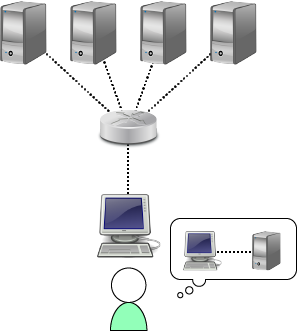
\includegraphics[clip,width=10.0cm]{images/sad.png}
			\caption{Sistema distribuído transparente}
			\label{fig:transparente}
		\end{center}
	\end{figure}
	
	
	O conceito de transparência pode ser aplicado os diversos aspectos de um sistema distribuído, os mais importantes são mostrado a seguir~\cite{tanenbaum07}:	

	\begin{itemize}
		
	\item\textbf{transparência de acesso} Não necessita fornecer a localização dos recursos, ou seja, os programas devem executar os processos de leitura/escrita de arquivos remotos da mesma maneira que operam sobre os arquivos locais, sem qualquer modificação no programa. O usuário não deve perceber se o recurso acessado é local ou remoto;
	
	\item\textbf{transparência de localização} Os programas clientes devem ver um espaço de nomes de arquivos uniforme, sem a necessidade de fornecer a localização física dos arquivos para encontrá-los, mesmo que esses arquivos se desloquem entre os servidores;
	
	\item\textbf{transparência de migração} Independente dos arquivos se moverem entre servidores, os programas clientes não precisam ser alterados para a nova localidade do grupo de arquivos. Essa característica permite flexibilidade em mover arquivos sem comprometer toda a estrutura, ou ter que refazer links entre programas clientes e o local do arquivo;
	
	\item\textbf{transparência de desempenho} O desempenho da aplicação cliente não poderá ser comprometido enquanto ocorre uma variação dos processos sobre os recursos disponíveis pelos SADs, isto é, mesmo que haja concorrência no acesso pelos arquivos isso não deve afetar os usuários;
	
	\item\textbf{transparência de escalabilidade} Os recursos computacionais podem sofrer alterações para abrigar maior poder computacional ou o ingresso de novos servidores sem prejudicar o serviço;
	
	\item\textbf{transparência a falhas} Visa garantir a disponibilidade dos arquivos ininterruptamente e se ocorrerem falhas o programa cliente não deverá saber como elas serão tratadas;
	
	\item\textbf{transparência de replicação}, Várias cópias dos mesmos arquivos armazenados em locais diferentes para garantir a disponibilidade. A aplicação cliente deverá
	visualizar apenas uma cópia do mesmo não necessitando saber a quantidade replicada e o local.
	
	\end{itemize}
	
	
	A transparência é altamente desejável em sistemas distribuídos, mas nem sempre é possível alcançá-la ou, em determinadas situações, não convém ocultá-la. Pode-se destacar uma situação que seja mais conveniente o usuário tomar uma decisão sobre
	alguma falha do que o sistema distribuído tentar resolver por si só. Isso pode ser observado quando um serviço, por repetidas vezes tenta estabelecer uma comunicação com o servidor na \textit{Internet}, neste caso o melhor é informar ao usuário sobre a falha e que ele tente mais tarde.
	
	
	
	%\begin{itemize}
	%\item Disponibilidade
	\subsection{Disponibilidade}
	A maioria dos SADs possuem serviços dependente da rede interna ou externa, onde ainda continua sendo um meio relativamente instável, podendo deixar o serviço fora de ar por causa de algum inconveniente que ocorreu na rede. 
	A sua arquitetura que possui grande quantidade de computadores constituindo o sistema também é um dos fatores que causam a indisponibilidade do serviço, pois a probabilidade de acontecer uma falha cresce de acordo com aumento do número de entidades envolvidas. 
	Foram feito vários estudos para evitar que os serviços deixem de ser oferecidos, independente de qual for a razão da inconveniência. 
	Assim, um SAD deve implementar um esquema para manter o acesso aos seus recursos em qualquer caso, estando sempre disponíveis para responder às requisições enviados por usuários. A falha que acontece em alguns servidores não pode influenciar a execução de serviço do sistema. 
	Além disso, o usuário não precisa saber como tal esquema funciona e nem como foi implementado, podendo continuar a usar o sistema sem preocupar com possíveis transtornos que estão acontecendo. 
	Essa restrição é incorporada para manter a propriedade de transparência do sistema.
	
	%\item Operações atômicas
	\subsection{Operação atômica}
	A operação atômica é um conjunto de operações que aparece para o resto do sistema como se fosse ocorrido instantaneamente.
	Quando um arquivo é submetido a este tipo de operação, o estado dele muda de um para outro sem apresentar outros estados intermediários durante a execução.
	Consequentemente, uma operação sobre arquivo é considerada atômica somente se as etapas que ela segue não são reconhecidas por outros processos que estão fora desta operação~\cite{tanenbaum07_2}. 
	Assim, para uma operação ser atômica deve satisfazer as seguintes condições.
	
	\begin{enumerate}
	\item Enquanto as etapas da operação estejam em progressão, nenhum entidade externa consegue perceber o estado intermediário desta operação.
	\item Uma operação é efetuada somente se todas as etapas dela são concluídas com sucesso, caso contrário, se tiver uma etapa que falhou, todas as etapas serão abortadas e o estado do sistema volta para antes de executá-la.
	\end{enumerate}
	
	Geralmente as operações de leitura, escrita, criação ou remoção de um arquivo apresentam propriedade atômica para maioria dos SAD.
	\\
	
	As transações são mecanismos que permitem realizar uma sequência de operações de forma atômica. Tais mecanismos disponibilizam determinados comandos para os usuários para que eles possam escolher quais operações serão executadas dentro de transações. Para montar uma transação, existem os comandos início e fim. O comando de início avisa ao sistema que todas as operações a partir daquele ponto estarão dentro da transação, e o comando de finalização indica que não virá mais nenhuma operação para aquela transação.
	Assim, caso alguma dessas operações falhe, o sistema desfaz, ou aborta, todas as alterações que as operações antes daquela realizaram. Isso é chamado de \textit{rollback} ou \textit{abort}. Caso todas as operações sejam executadas sem problemas ou erros, ao chegar no fim da transação é realizado um \textit{commit}, ou seja, todas as alterações que foram executadas são efetivadas e persistidas, de tal forma que outros processo possam percebê-las. Com isso as transações implementam a semântica do tudo ou nada, ou seja, ou todas as operações são executadas com sucesso, ou nenhuma será executada. Isso faz das transações um importante mecanismo de tolerância a falhas, pois elas evitam que pequenas falhas prejudiquem a integridade de todo o sistema.
	
	%\item Tolerância a falhas e gerenciamento de falhas
	\subsection{Tolerância a falhas e gerenciamento de falhas}
	O sistema deve ser capaz de continuar com sua operação normal mesmo que um ou mais componentes apresentam falha, isolando esses componentes.
	Durante a transmissão dos dados entre servidores e clientes, podem ocorrer falhas, seja por excesso de tráfego de pacotes pela rede, seja por algum dos servidores estar sobrecarregado. 
	Além disso, podem ocorrer falhas de \textit{hardware}, especialmente dos mecanismos de armazenamento, de transmissão e entre outros. 
	Esses problemas acontecem em grande parte porque os sistemas distribuídos são implementados sobre redes de computadores que não são totalmente confiáveis. 
	É por causa disso que a maior parte da complexidade de sua implementação está em levar em conta esse ambiente propício a falhas. 
	Um sistema distribuído precisa usar um protocolo de comunicação com capacidade para detecção de erros de transmissão~\cite{kon94}. Assim, caso uma mensagem chegue alterada no seu destino, o protocolo precisa perceber isso e retransmiti-la. 
	Isso deve ocorrer também para mensagens que se perderam no caminho.
	Um outro problema que a rede pode ter é o seu particionamento por tempo indeterminado. 
	Mas não é só com a rede que devemos nos preocupar, em que o \textit{hardware} dentro das máquinas também pode apresentar falhas. 
	Por exemplo, um disco rígido pode deixar de funcionar de um momento para outro, seja por excesso de uso ou até mesmo por descargas elétricas. 
	Nesse caso pode-se criar soluções desde redundância física do equipamento, realizada via \textit{hardware}, ou redundância controlada pelo próprio sistema distribuído, que cuidaria de replicar os dados, para evitar a perda dos mesmos.
	\\
	 
	Seja qual for o problema, o sistema deve evitar que o cliente fique aguardando uma resposta por muito tempo, ou que seus dados sejam danificados ou até mesmo perdidos. Isso significa que o serviço precisa ter disponibilidade e confiabilidade.
	Porém, muitas vezes essas características se conflitam. Por exemplo, uma forma de garantir a confiabilidade é implementar redundância dos dados, porém a complexidade que isso gera pode aumentar demais a carga do servidor, comprometendo a disponibilidade, pois as respostas aos clientes seriam mais lentas.
	Outro mecanismo que auxilia a confiabilidade é a transação. Ela evita que o conteúdo de algum arquivo fique em um estado inconsistente caso haja uma queda do servidor ou cliente durante a execução de alguma operação sobre o mesmo.
	\\
	
	Das falhas pode-se destacar os seguintes problemas:
	\begin{itemize}
		\item \textbf{falha por queda}, problema físico ou lógico no servidor, causando o travamento do sistema operacional;
		
		\item \textbf{falha por omissão}, significa o não recebimento das mensagens, quer seja por causa de mensagens não aceitas ou por não enviar uma resposta depois da ação concluída;
		
		\item \textbf{falha de temporização}, ocorre quando uma reposta está fora do intervalo de tempo adequado;
		
		\item \textbf{falha de resposta} consiste da resposta emitida estar incorreta, ou seja, o retorno não condiz com a solicitação;
		
		\item \textbf{falha arbitrária}, também conhecida como falha bizantina, ocorre quando um
		servidor envia mensagens inadequadas, mas que não são consideradas como incorretas.
		Também pode ser associada a um servidor que está atuando maliciosamente
		e, portanto, emitindo respostas erradas de forma proposital.
		
	\end{itemize}
	
	%\item Replicação de arquivos
	\subsection{Replicação de arquivos}
	No contexto de SAD, a abordagem de replicação tem dois motivos para ser utilizada. 
	Um deles é a distribuição da carga de acesso entre todos os servidores que constitui o sistema. 
	Se existir um arquivo que é acessado por clientes com alta frequência, a transmissão concentra no servidor que armazena tal arquivo, causando sobrecarga neste servidor e consumo excessivo da banda dessa conexão, o que resulta na degradação de desempenho do sistema todo. 
	Para evitar a concentração de acesso, um solução trivial pode ser adotada é criar algumas cópias de arquivos, geralmente três, e distribuir ao longo dos servidores para descentralizar os acessos. \\
	
	
	Além disso, se um sistema de arquivos oferece essa funcionalidade, a confiança do serviço de arquivos é generosamente aumentada.
	Caso um determinado servidor caia ou fique indisponível, o serviço de arquivos ainda pode continuar com suas operações por possuir cópias dos dados em outro ponto da rede.
	Assim, replicação de arquivos provê tolerância a falhas, já que o usuário nem sequer percebe que o servidor que ele estava usando caiu e qual outro entrou no lugar para prover o recurso que ele estava usando. Por isso o sistema também deve oferecer transparência de replicação pois o usuário não precisa saber como o sistema cuida da replicação desse arquivo.
	O maior problema nessa característica do SAD é que a implementação pode ser muito complicada, pois é necessário manter os dados sincronizados e consistentes ao mesmo tempo.
	Existem dois tipos de implementações: a primeira utiliza comunicação em grupo, que consiste em quando ocorrer uma alteração por algum dos servidores, este manda por \textit{broadcast} para os outros servidores dizendo que o arquivo foi alterado. Estes, por
	sua vez, podem alterar esse arquivo imediatamente ou somente quando forem utilizá-lo; a segunda utiliza votação e números de versão. Isso significa que quando um cliente pedir permissão para alterar um arquivo, os servidores votarão entre eles pra saber quem possui a versão mais recente, e esse servidor será o servidor padrão daquele arquivo, e seu número de versão será incrementado. Todas essas ideias, além de serem complicadas de implementar, geram alguns problemas. Manter a sincronização entre os servidores, para o caso de alterações no sistema de arquivos, é uma delas.
	
	
	%\item Escalabilidade
	\subsection{Escalabilidade}
	%- capacidade de aumentar o desempenho do sistema com adição de recurso.
	Os sistemas distribuídos são, em geral, projetados e configurados pensando-se na configuração da rede naquele momento. 
	Pode acontecer dessa rede aumentar, ou seja, dezenas ou centenas de novos nós serem adquiridos e conectados nesse sistema. 
	A menos que se tenha pensado nessa situação no momento do projeto dessa rede, dificilmente um SAD apresentará bom desempenho para servir todos esses clientes após um crescimento tão grande da rede. 
	Vários problemas podem ocorrer, como, por exemplo, quando o servidor responde a um pedido de um cliente e mantém esses dados enviados em \textit{cache}, para permitir uma rápida resposta caso esse mesmo dado seja requisitado novamente. 
	No caso de se ter muitos clientes, ocorrerá de se ter muitos pedidos diferentes, fazendo com que as tabelas do \textit{cache} sejam atualizadas com frequência, sem a reutilização dos dados lá contidos. 
	Isso acabará causando uma sobrecarga do sistema, pois por ter muitos clientes, muitas requisições serão feitas em um curto intervalo de tempo, e os dados que estavam no \textit{cache} rapidamente serão trocados por outros requisitados por outros clientes. 
	Caso se tenha \textit{cache} do lado dos clientes, ao se alterar um arquivo que está sendo usado por muitas outras máquinas, o servidor terá que avisá-las que o \textit{cache} local das mesmas está inválido, e todas deverão atualizar com a versão do servidor, causando mais sobrecarga. 
	\\
	
	Por outro lado, caso se tenha estimado que a rede seria muito grande e se tenha distribuído o sistema de arquivos em muitos servidores, fica difícil descobrir onde um arquivo está armazenado fisicamente. 
	Por exemplo, se para abrir um arquivo um cliente tiver que perguntar para cada servidor se ele é o responsável por aquele arquivo, certamente haverá um congestionamento na rede. 
	Caso se tente resolver isso colocando um servidor central para resolver todos os caminhos para os arquivos, indicando a localização do mesmo, tal servidor sofrerá sobrecarga. 
	Um sistema escalável é um sistema que leva em conta esses problemas e tenta evitar sua ocorrência quando o número de clientes aumenta extremamente.
	
	%\item Acesso concorrente
	\subsection{Acesso concorrente}
	%- deve ser possível o acesso compartilhado aos recursos.
	Vários usuários podem acessar vários arquivos, ou os mesmos arquivos, sem sofrer danos, perda de desempenho ou quaisquer outras restrições. Isso tudo deve ocorrer sem que o usuário precise saber como o acesso é realizado pelos servidores. Assim, é necessário haver transparência de concorrência.
	O maior problema encontrado nas implementações desse tipo de solução é quanto à sincronização dos arquivos, o que inclui leitura e escrita concorrente. A leitura concorrente pode ser implementada facilmente se não houver escrita concorrente, pois quando um arquivo estiver sendo lido, certamente ninguém poderá escrever nele. 
	Caso também se queira escrita concorrente, deve-se levar em conta que quando um cliente escreve em um arquivo, todos os leitores devem ser avisados que o arquivo foi alterado, e todos escritores precisam tomar cuidado para não escrever em cima das alterações que foram feitas por outros.
	Assim, ou vale a última alteração, ou os escritores discutem entre si para tentar fundir as alterações de uma forma adequada.
	\\
	
	Para se ter uma idéia de como esse problema é complexo, imagine duas operações bancárias ocorrendo simultaneamente para a mesma conta. Uma delas é um saque de R\$200,00 e outra é um depósito de R\$1000,00. Antes dessas operações, suponha que essa conta possua R\$100,00 de saldo, e também suponha que esse valor esteja armazenado em um arquivo de um SAD desse sistema bancário. Quando o cliente da conta for realizar o saque, a aplicação irá armazenar em memória o valor atual do saldo, assim como acontecerá com a aplicação do outro caixa que estará recebendo o depósito. Esta aplicação, então, irá adicionar ao saldo o valor do depósito, e gravará no arquivo o novo saldo, que será de R\$1200,00. Porém, a primeira aplicação irá subtrair do valor armazenado em memória, que para seu contexto é de R\$100,00, o valor do saque, e gravará o resultado, o valor R\$100,00, no mesmo arquivo, sobrescrevendo o valor lá existente. Dessa forma, o cliente perderia seu depósito.\\
	
	Para evitar esse tipo de problema, as aplicações que operam dessa forma podem agrupar um conjunto de operações no sistema de arquivos como sendo uma única transação, deixando a cargo do sistema operacional gerenciar a melhor forma de executar isso.
	Existem alguns mecanismos para o controle dessa concorrência. Dentre eles, destaca-se o mecanismo de \textit{locks}, por ser o mais amplamente utilizado. Tal sistema de controle de concorrência baseia-se no bloqueio do arquivo que se quer acessar antes de acessá-lo, através de uma chamada ao sistema operacional. Caso um segundo processo queira usar o mesmo arquivo, ele tentará realizar o bloqueio, usando o mesmo comando que o primeiro processo, e o sistema operacional o avisará que esse arquivo já está bloqueado. Cabe ao processo decidir se espera na fila pelo desbloqueio ou se continua seu processamento sem o acesso ao arquivo. Esse desbloqueio é realizado pelo processo detentor do arquivo, através de um comando do sistema operacional, assim
	como foi feito o bloqueio.\\
	
	Através desses bloqueios, é possível tornar as transações serializáveis, isto é, o resultado da operação de várias transações simultâneas é o mesmo obtido se elas fossem realizadas uma após a outra~\cite{kon94}. Um protocolo para a realização dessa serialização seria o protocolo de bloqueio de duas fases, onde na primeira fase ocorreria o bloqueio de todos os arquivos a serem usados nessa transação, e na segunda fase seria a liberação conjunta de todos os arquivos, após a realização das operações dentro dessas fases.
	Porém esse protocolo pode gerar um \textit{deadlock}, onde algum processo esperaria a liberação de um arquivo que foi bloqueado por outro processo, que também estaria esperando a liberação de um arquivo que foi bloqueado por aquele primeiro processo, por exemplo.
	
	%\item Segurança
	\subsection{Segurança}
	Os recursos devem ser protegidos contra acessos ilegais, permitindo somente a execução das operações solicitadas de um usuário conhecido. 
	Compartilhar arquivos entre vários ambientes e usuários é uma das vantagens que os sistemas de arquivos distribuídos nos trazem. Porém, deixar que outras pessoas possam acessar arquivos confidenciais, como, por exemplo, extrato de conta bancária, é um grande problema. 
	Dessa forma, torna-se necessário adotar mecanismos de segurança, para evitar que pessoas desautorizadas tenham acesso aos arquivos do sistema. 
	\\
	
	
	Sistemas como Unix\textit{Unix} adotam um método baseado em permissões para controlar o acesso aos seus arquivos.
	Cada arquivo possui informações sobre quais usuários podem acessá-lo e de que maneira.
	Nos sistemas distribuídos que rodam sob o \textit{Unix}, quando um servidor recebe um pedido para enviar dados de um determinado arquivo, ele também recebe informações sobre qual usuário está tentando realizar tal acesso. Com isso, verifica se tal usuário tem permissão suficiente para realizar essa solicitação, fazendo uma comparação com as informações de permissões do arquivo.
	Além disso, os sistemas \textit{Unix} possuem um usuário chamado \textit{root}, que possui permissão para acessar todos os arquivos da máquina local, de forma ilimitada. Isso funciona bem em sistemas locais, mas em uma rede já começam a surgir os problemas.
	Por exemplo, pode-se configurar as máquinas vizinhas de uma rede para confiarem no usuário \textit{root} entre elas. Assim, um usuário \textit{root} de uma máquina pode acessar os arquivos de outra máquina como se fosse o usuário \textit{root} local. O problema é se um usuário mal-intencionado consegue acesso como \textit{root}. Dessa forma ele teria acesso a todas as máquinas da rede. Outro problema é se o pedido que vier da rede for alterado para que o servidor acredite que quem está pedindo é ou o dono do arquivo ou o \textit{root}. Dessa forma, pode-se acessar qualquer arquivo da rede também. \\
	
	Outra forma de implementar esse controle de segurança é um sistema baseado em capacidades, que consiste de o cliente enviar ao servidor uma prova de que ele possui a capacidade de acessar um determinado arquivo. Na primeira vez que o usuário acessa tal arquivo, é enviado ao servidor sua identificação, e o servidor por sua vez retorna um código que é a sua prova de capacidade para acessar aquele arquivo. Nas próximas requisições, o cliente não precisa mais se identificar, bastando apenas enviar a prova de sua capacidade. Deve-se tomar cuidado para não criar provas de capacidade que sejam fáceis de serem forjadas. Até agora comentamos sobre o controle no acesso aos arquivos. Porém, caso haja outras máquinas no caminho de duas máquinas confiáveis, existe o risco de se ter dados interceptados ou, até mesmo, adulterados. Uma forma de se resolver esse problema é criptografar as informações antes de enviá-las.
	
	%\item Heterogeneidade
	%\subsubsection{Heterogeneidade}
	%No sistema distribuído que apresenta heterogeneidade o seu funcionamento não é afetado por diferenças em sistemas operacionais, protocolos de comunicação, linguagens de programação, formatos de dado e arquiteturas de hardware. 
	
	
	%\item Extensibilidade e abertura
	%\subsubsection{Extensibilidade e abertura}
	%Os interfaces devem ser claramente separados e publicamente disponíveis para facilitar o adicionamento de novos componentes e as extensões para componentes existentes.
	
	%\item Migração e balanceamento de carga
	%\subsubsection{Migração e balanceamento de carga}
	%Permitir a circulação de tarefas dentro de um sistema, sem afetar a operação do usuário ou aplicativos, e distribuir a carga entre os recursos disponíveis para melhorar o desempenho.
	
	
	
	%\end{itemize}
		
	\subsection{Nomes e localização}
	Todo arquivo armazenado em um sistema de arquivos possui um nome e um caminho, que o identifica unicamente em tal sistema.
	Um caminho representa um nó de uma estrutura de diretórios, que pode ser representada como uma árvore como mostra na Figura~\ref{fig:arv_dir}.
	Tal árvore possui uma raiz, e cada nó pode possuir mais árvores ou arquivos.
	Dessa forma, para localizar um arquivo em uma árvore de diretórios basta seguir o caminho do arquivo, e ao chegar no diretório final procurar pelo nome de tal arquivo.
	A forma como esse nome e esse caminho são definidos dependem muito do sistema operacional. 
	Por exemplo, no \textit{Unix} um caminho é definido como uma sequência de nomes de diretórios, todos separados pelo caractere "/". O último nome dessa sequência pode ser o nome do arquivo, ou de um diretório, caso se esteja definindo um caminho para o mesmo.
	Em sistemas distribuídos, é possível que se encontre o nome da máquina em que o arquivo se encontra dentro dessa definição de caminho. Porém procura-se deixar isso transparente para o usuário.
	
	\begin{figure}[htb]
		\begin{center}
			
			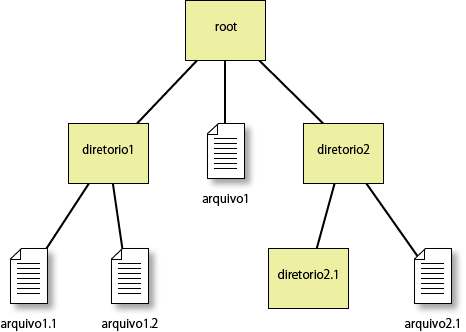
\includegraphics[clip,width=10.0cm]{images/image3.png}
			\caption{Árvore de diretórios}
			\label{fig:arv_dir}
		\end{center}
	\end{figure}
	

	\section{Conclusões do Capítulo}
	Neste capítulo foi introduzido o que é um sistema de arquivos distribuído. 
	Algumas propriedades do sistema, tais como operação atômica, tolerância a falhas ou acesso concorrente, serão implementados utilizando a biblioteca \textit{BFT-SMaRt}, o que será apresentado mais adiante no Capítulo 4.
 

	

